\documentclass[conference]{IEEEtran}
\IEEEoverridecommandlockouts
\usepackage{cite}
\usepackage{amsmath,amssymb}
\usepackage{graphicx}
\usepackage{booktabs}
\usepackage{multirow}
\usepackage{xcolor}
\usepackage{tikz}
\usetikzlibrary{arrows.meta,positioning,fit}
\usepackage[hidelinks]{hyperref}
\usepackage{url}
\def\BibTeX{{\rm B\kern-.05em{\sc i\kern-.025em b}\kern-.08em
    T\kern-.1667em\lower.7ex\hbox{\sc e}\kern-.125emX}}

\begin{document}

\title{Quantifying Vendor Lock-In in Multi-Cloud Infrastructure: A Static-Analysis Lock-In Index and an Empirical Study of 677 Terraform Configurations}

\author{
\IEEEauthorblockN{Deepak Soni}
\IEEEauthorblockA{\textit{Dept. of Computer Science \& Engg.} \\
\textit{[Institution Name]}\\
{}[City], India \\
ID: 590012874}
\and
\IEEEauthorblockN{Navneet Pant}
\IEEEauthorblockA{\textit{Dept. of Computer Science \& Engg.} \\
\textit{[Institution Name]}\\
{}[City], India \\
ID: 590011569}
\and
\IEEEauthorblockN{Mohd Toshif}
\IEEEauthorblockA{\textit{Dept. of Computer Science \& Engg.} \\
\textit{[Institution Name]}\\
{}[City], India \\
ID: 590018042}
}

\maketitle

\begin{abstract}
Vendor lock-in is one of the most cited obstacles to multi-cloud adoption, yet practitioners still judge it mostly by intuition. This paper proposes the Lock-In Index (LII), a 0--100 score that estimates how tightly an Infrastructure-as-Code (IaC) configuration is bound to a single cloud provider. Each declared resource is mapped to one of 21 service categories, and each category is scored on four dimensions: API proprietariness, data and state lock, the gap to functionally equivalent services elsewhere, and egress exposure. We implement the index as a static analyzer for Terraform and apply it to 677 root configurations (8{,}908 resource declarations, 844 distinct resource types) drawn from 23 public repositories covering AWS, Azure, and Google Cloud. Three findings stand out. First, ``glue'' resources---identity and access management, networking, governance, secrets, and observability---make up 59.7\% of all resources and 52.7\% of the measured lock-in, with IAM alone contributing more lock-in than any application service. Second, configurations built around managed Platform-as-a-Service (PaaS) components score far higher (median 41.9) than Kubernetes-centric ones (median 25.2; Cliff's $\delta=-0.84$, $p<10^{-18}$). Third, configuration rankings remain stable when rubric weights and scores are randomly perturbed (median Spearman $\rho=0.91$ over 1{,}000 trials). We also show that list-price egress for a full exit grows from roughly \$850--1{,}100 at 10~TB to \$48{,}000--80{,}000 at 1~PB, and discuss how recent provider waivers and the EU Data Act change that picture. The analyzer, rubric, and data are released to support replication.
\end{abstract}

\begin{IEEEkeywords}
vendor lock-in, multi-cloud, cloud portability, infrastructure as code, Terraform, static analysis, migration cost
\end{IEEEkeywords}

\section{Introduction}

Moving an application from one public cloud to another is rarely as simple as redeploying it. Over time, an application accumulates dependencies on provider-specific services: a managed key--value store with its own query model, an identity system with its own policy language, event triggers that exist only on one platform. Each dependency raises the cost of leaving. This condition, commonly called \emph{vendor lock-in}, has been identified repeatedly as a major barrier to cloud adoption and to multi-cloud strategies~\cite{opara2014,opara2016,silva2013}.

Despite the attention it receives, lock-in is still discussed mostly in qualitative terms. Surveys establish that organizations worry about it~\cite{opara2016}, and systematic reviews catalogue the techniques proposed to avoid it~\cite{silva2013}, but an architect who wants to know \emph{how locked-in a particular system is} has few tools to answer the question. Standards such as TOSCA~\cite{tosca,binz2012} and abstraction layers such as Kubernetes~\cite{burns2016} promise portability, but their effect is rarely measured on real deployments.

At the same time, Infrastructure-as-Code (IaC) has made cloud architectures machine-readable. Tools such as Terraform describe every provisioned resource declaratively, and thousands of such descriptions are publicly available~\cite{buehler2025}. This creates an opportunity: if lock-in can be expressed as a function of the resources an application declares, it can be measured automatically and at scale.

This paper makes four contributions:
\begin{enumerate}
\item A \textbf{Lock-In Index (LII)} that scores each resource on four dimensions of portability and aggregates the scores to the configuration level (Section~\ref{sec:method}).
\item A \textbf{static analyzer} for Terraform that resolves local modules, classifies resource types into 21 service categories, and computes the index.
\item An \textbf{empirical study} of 677 root configurations from 23 public repositories, answering four research questions about where lock-in comes from and how robust the measurement is (Section~\ref{sec:results}).
\item An \textbf{exit-cost analysis} that combines published egress prices with recent regulatory and commercial changes (Section~\ref{sec:egress}).
\end{enumerate}

We address the following research questions:
\begin{itemize}
\item \textbf{RQ1:} How is lock-in distributed across configurations and providers?
\item \textbf{RQ2:} Which service categories contribute most to lock-in?
\item \textbf{RQ3:} Does the index separate architectural styles that are expected to differ in portability?
\item \textbf{RQ4:} How sensitive are the results to the rubric's weights and scores?
\end{itemize}

\section{Background and Related Work}
\label{sec:related}

\subsection{Vendor Lock-In and Cloud Portability}
Opara-Martins \textit{et al.}~\cite{opara2014} reviewed the business, technical, and legal dimensions of lock-in and argued that limited interoperability between providers is its root cause. Their later survey of 114 participants found that lock-in risk grows as computing moves from on-premise infrastructure to the cloud, and recommended favouring vendors that support standard data formats and APIs~\cite{opara2016}. Silva \textit{et al.}~\cite{silva2013} systematically reviewed proposed lock-in solutions and observed that most are technology-oriented and evaluated only lightly. Petcu~\cite{petcu2011} distinguished portability (moving an application) from interoperability (making services work together) and surveyed the approaches available for each. Satzger \textit{et al.}~\cite{satzger2013} proposed a ``meta cloud'' that would let applications be deployed across providers through a common abstraction layer.

These studies frame the problem well, but none offers a metric that can be computed for a concrete system. Our work complements them by turning several of their qualitative criteria---standard APIs, open data formats, availability of alternatives---into scored dimensions.

\subsection{Standards and Abstraction Layers}
TOSCA, an OASIS specification, describes application topologies and their management plans in a provider-neutral way~\cite{tosca}. Binz \textit{et al.} showed how TOSCA plans can make operational aspects portable~\cite{binz2012,binz2014}. Brogi \textit{et al.}~\cite{brogi2014} noted, however, that TOSCA makes \emph{descriptions} of applications portable, not the applications themselves. Kubernetes, which grew out of Google's Borg and Omega systems~\cite{burns2016}, offers a different route: a common container-orchestration API that every major provider now hosts as a managed service. Whether such layers reduce lock-in in practice is one of the questions our index is designed to answer.

\subsection{Empirical Studies of Infrastructure as Code}
Rahman \textit{et al.}~\cite{rahman2019} mapped IaC research and found that most work at the time addressed frameworks and tools rather than empirical quality. More recent studies mine public Terraform code: Verdet \textit{et al.}~\cite{verdet2025} measured the adoption of security policies across AWS, Azure, and Google Cloud repositories; Feitosa \textit{et al.}~\cite{feitosa2023} looked for evidence of cost awareness in IaC artifacts; and Buehler \textit{et al.}~\cite{buehler2025} released TerraDS, a dataset of tens of thousands of permissively licensed Terraform repositories. To our knowledge, no prior study has used IaC to measure vendor lock-in.

\section{The Lock-In Index}
\label{sec:method}

\subsection{Design Rationale}
A useful lock-in metric should be (i) computable from artifacts that teams already maintain, (ii) interpretable at the level of individual resources, so that engineers know what to change, and (iii) transparent enough that its assumptions can be debated and revised. We therefore chose a rubric-based design over a learned model: every number in the index can be traced to an explicit score in Table~\ref{tab:rubric}.

\subsection{Dimensions}
Each resource $r$ is assigned a service category $c(r)$. Each category is scored on four dimensions, each in $[0,1]$:
\begin{itemize}
\item \textbf{API proprietariness ($A$):} how far the service's interface and semantics are specific to one provider. An S3-compatible object API scores low; a provider's IAM policy language scores high.
\item \textbf{Data and state lock ($D$):} how difficult it is to export the state the resource holds in a usable form. Stateless resources score zero.
\item \textbf{Equivalence gap ($E$):} how far the closest equivalent on another provider, or an open-source substitute, is from a drop-in replacement.
\item \textbf{Egress exposure ($X$):} how much bulk data the resource typically holds and would have to transfer out on exit.
\end{itemize}

\subsection{Aggregation}
The resource-level score is a weighted sum,
\begin{equation}
\mathrm{LII}(r) = w_A A_{c(r)} + w_D D_{c(r)} + w_E E_{c(r)} + w_X X_{c(r)},
\label{eq:res}
\end{equation}
with default weights $w=(0.35,\,0.25,\,0.25,\,0.15)$. API proprietariness receives the largest weight because rewriting integration code is usually the dominant engineering cost of a migration; egress receives the smallest because it is a one-time, largely predictable expense (Section~\ref{sec:egress}). For a configuration $C$ with provider resources $R_C$, the index is the mean resource score scaled to 0--100:
\begin{equation}
\mathrm{LII}(C) = \frac{100}{|R_C|}\sum_{r\in R_C}\mathrm{LII}(r).
\label{eq:cfg}
\end{equation}
We use a mean rather than a sum so that the index describes the \emph{character} of a configuration and is not dominated by its size. To attribute lock-in to categories across a corpus, we define the lock-in mass of category $k$ as $M_k=\sum_C\sum_{r\in R_C,\,c(r)=k}\mathrm{LII}(r)$ and report each category's share $M_k/\sum_j M_j$.

\begin{table}[t]
\caption{Scoring rubric: dimension scores per service category and resulting resource-level LII (default weights).}
\label{tab:rubric}
\centering
\footnotesize
\setlength{\tabcolsep}{3.2pt}
\begin{tabular}{@{}lccccr@{}}
\toprule
Category (example resources) & $A$ & $D$ & $E$ & $X$ & LII \\
\midrule
Proprietary NoSQL (DynamoDB, Cosmos DB) & .9 & .8 & .7 & .8 & 81.0 \\
Analytics/AI (BigQuery, SageMaker) & .9 & .7 & .6 & .9 & 77.5 \\
API/workflow (API Gateway, Logic Apps) & .9 & .2 & .6 & 0 & 51.5 \\
Raw ARM API (\texttt{azapi\_*}) & .9 & .2 & .5 & .1 & 50.5 \\
Messaging/eventing (SQS, Pub/Sub) & .8 & .3 & .4 & .2 & 48.5 \\
IAM/identity (roles, policies) & .9 & 0 & .5 & 0 & 44.0 \\
Serverless functions (Lambda) & .8 & .1 & .4 & 0 & 40.5 \\
Observability (CloudWatch) & .7 & .2 & .3 & .1 & 38.5 \\
Governance/org (projects, policies) & .8 & 0 & .4 & 0 & 38.0 \\
Other provider (unclassified) & .6 & .2 & .4 & .1 & 37.5 \\
Proprietary containers (ECS, Cloud Run) & .7 & .1 & .4 & 0 & 37.0 \\
Secrets/KMS & .6 & .3 & .3 & 0 & 36.0 \\
Object storage (S3, GCS, Blob) & .3 & .3 & .1 & .9 & 34.0 \\
Relational DB (RDS, Cloud SQL) & .3 & .4 & .1 & .7 & 33.5 \\
Block storage (EBS, managed disks) & .2 & .4 & .1 & .5 & 27.0 \\
Edge (LB, DNS, CDN) & .5 & 0 & .3 & .1 & 26.5 \\
Compute (VMs, autoscaling) & .3 & .2 & .1 & .2 & 21.0 \\
Network core (VPC, subnets, routes) & .4 & 0 & .2 & 0 & 19.0 \\
Container registry (ECR, ACR) & .2 & .2 & .1 & .3 & 19.0 \\
Managed Kubernetes (EKS, AKS, GKE) & .3 & .1 & .1 & .1 & 17.0 \\
Kubernetes-native (\texttt{kubernetes\_*}, \texttt{helm\_*}) & .1 & .1 & 0 & 0 & 6.0 \\
\bottomrule
\end{tabular}
\end{table}

\subsection{Static Analyzer}
Fig.~\ref{fig:pipeline} summarizes the pipeline. The analyzer identifies \emph{root configurations}---directories that are deployed directly, such as module examples, sample applications, and landing-zone stages. For each root, it extracts \texttt{resource} blocks from every \texttt{.tf} file and recursively follows \texttt{module} blocks whose source is a local path, so that resources hidden inside local modules are counted. The provider is derived from the resource-type prefix (\texttt{aws\_}, \texttt{azurerm\_}/\texttt{azuread\_}/\texttt{azapi\_}, \texttt{google\_}). Utility providers that create no cloud infrastructure (\texttt{random}, \texttt{null}, \texttt{tls}, \texttt{time}, and similar) are excluded. Resource types are mapped to categories by an ordered list of regular-expression rules; resources of the Kubernetes and Helm providers form their own low-lock-in category because their API is the same on every managed cluster.

\begin{figure}[t]
\centering
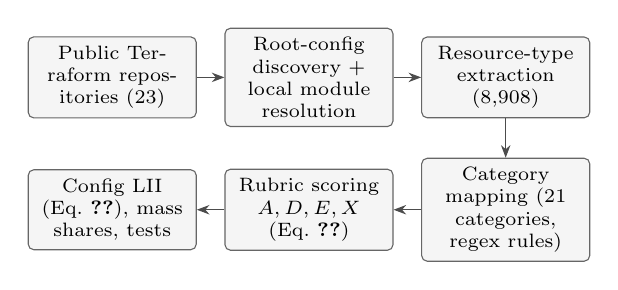
\begin{tikzpicture}[
  node distance=3.5mm,
  box/.style={draw=black!60, rounded corners=2pt, fill=black!4, align=center,
              font=\scriptsize, minimum height=7.5mm, text width=19mm},
  arr/.style={-{Stealth[length=1.6mm]}, black!70}]
\node[box] (a) {Public Terraform repositories (23)};
\node[box, right=of a] (b) {Root-config discovery + local module resolution};
\node[box, right=of b] (c) {Resource-type extraction (8{,}908)};
\node[box, below=5mm of c] (d) {Category mapping (21 categories, regex rules)};
\node[box, left=of d] (e) {Rubric scoring $A,D,E,X$ (Eq.~\ref{eq:res})};
\node[box, left=of e] (f) {Config LII (Eq.~\ref{eq:cfg}), mass shares, tests};
\draw[arr] (a) -- (b); \draw[arr] (b) -- (c); \draw[arr] (c) -- (d);
\draw[arr] (d) -- (e); \draw[arr] (e) -- (f);
\end{tikzpicture}
\caption{Analysis pipeline used to compute the Lock-In Index.}
\label{fig:pipeline}
\end{figure}

\section{Study Design}
\label{sec:design}

\subsection{Corpus}
We built the corpus from 28 public GitHub repositories, cloned on October 29, 2026. They were chosen to cover the three largest providers and a range of architectural styles: official provider example directories (\texttt{hashicorp/terraform-provider-aws}, \texttt{-azurerm}), widely used community and vendor module collections (\texttt{terraform-aws-modules}, \texttt{terraform-google-modules}, Azure Verified Modules), Google's documentation samples, the AWS \texttt{serverless-patterns} collection, Google's Cloud Foundation Fabric, and HashiCorp's tutorial repositories for EKS, AKS, and GKE. One framework (\texttt{aztfmod/terraform-azurerm-caf}) was excluded because it is driven by variable files rather than resource declarations, and four repositories yielded no qualifying configuration, mainly because they consume modules from the Terraform registry, which the analyzer does not expand. A root configuration was retained if it declared at least three provider resources after module resolution. The final corpus contains 677 configurations from 23 repositories: 191 AWS, 248 Azure, and 238 Google Cloud. They declare 8{,}908 resources of 844 distinct types; only 1.3\% of declarations fell into the unclassified category. The median configuration declares six resources. No configuration declared resources for more than one of the three providers, a point we return to in Section~\ref{sec:discussion}.

\subsection{Architectural Groups for RQ3}
To test whether the index behaves as expected, each configuration was placed in one of three groups. \emph{Kubernetes-centric} configurations use managed Kubernetes or Kubernetes/Helm resources and no proprietary PaaS. \emph{Managed-PaaS-centric} configurations use at least one of serverless functions, proprietary NoSQL, API/workflow services, or proprietary container platforms, and no Kubernetes. All others are \emph{IaaS/other}. No configuration in the corpus combined Kubernetes with these PaaS categories, so no mixed group was needed. Group differences were tested with the two-sided Mann--Whitney $U$ test, and effect size is reported as Cliff's $\delta$.

\subsection{Sensitivity Analysis for RQ4}
Because the rubric reflects expert judgment, we ran 1{,}000 Monte Carlo trials. In each trial, weights were drawn from a Dirichlet distribution centred on the defaults (concentration 4), and every category score was shifted by an independent uniform perturbation in $[-0.15, 0.15]$, clipped to $[0,1]$. We then measured the Spearman correlation between the perturbed and baseline rankings of configurations and of categories.

\section{Results}
\label{sec:results}

\subsection{RQ1: Distribution Across Configurations and Providers}

\begin{table}[t]
\caption{Corpus composition and LII by dominant provider.}
\label{tab:corpus}
\centering
\footnotesize
\begin{tabular}{@{}lrrrcc@{}}
\toprule
Provider & Configs & Repos & Mean & Median & IQR \\
\midrule
AWS   & 191 & 10 & 38.6 & 41.5 & 34.1--44.4 \\
Azure & 248 & 5  & 31.1 & 27.2 & 24.3--37.3 \\
GCP   & 238 & 8  & 31.8 & 28.6 & 23.6--38.4 \\
\midrule
All   & 677 & 23 & 33.5 & 33.5 & --- \\
\bottomrule
\end{tabular}
\end{table}

\begin{figure}[t]
\centering
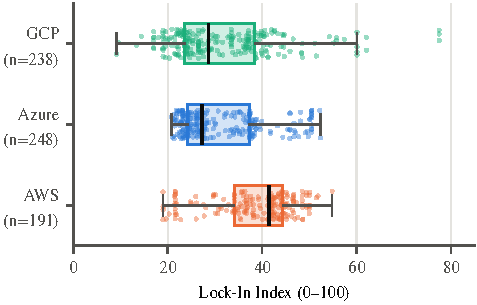
\includegraphics[width=\columnwidth]{figs/fig_provider.pdf}
\caption{Distribution of the Lock-In Index by dominant provider. Boxes show the interquartile range; points are individual configurations.}
\label{fig:provider}
\end{figure}

Table~\ref{tab:corpus} and Fig.~\ref{fig:provider} show the distribution. Scores range from 9.1 to 77.5, and 27.2\% of configurations exceed 40. AWS configurations score higher than both Azure (Cliff's $\delta=0.43$, $p<10^{-14}$) and Google Cloud ($\delta=0.42$, $p<10^{-13}$), while Azure and Google Cloud are indistinguishable ($\delta=0.00$, $p=0.96$).

We caution against reading this as a statement about the providers themselves. The AWS sample includes 90 configurations from \texttt{serverless-patterns}, whose median is 44.1; even without them, the AWS median is 36.7, but the remaining AWS repositories are also weighted toward Lambda, DynamoDB, and API Gateway modules. The provider difference is better explained by \emph{what the sampled code builds} than by the provider. Configuration size is only weakly related to the index (Spearman $\rho=0.13$), confirming that the mean-based aggregation does not simply reward larger deployments.

\subsection{RQ2: Which Categories Drive Lock-In}

\begin{figure}[t]
\centering
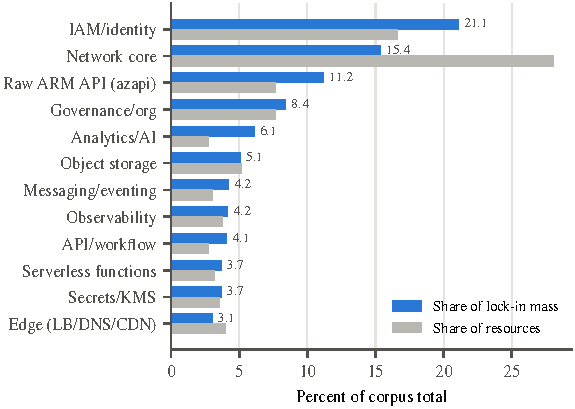
\includegraphics[width=\columnwidth]{figs/fig_categories.pdf}
\caption{Share of resources and share of total lock-in mass for the twelve largest categories. Categories whose blue bar exceeds their grey bar contribute more lock-in than their frequency alone suggests.}
\label{fig:categories}
\end{figure}

Fig.~\ref{fig:categories} compares each category's share of resources with its share of lock-in mass. The largest single source of lock-in is not a database or a serverless runtime but \textbf{identity and access management}: IAM resources are 16.6\% of all declarations, appear in 38.6\% of configurations, and account for 21.1\% of the lock-in mass. Every role, policy, and binding encodes the provider's permission model, and none of it transfers to another cloud without being rewritten.

Taken together, the ``glue'' categories---IAM, network core, governance, secrets, and observability---make up 59.7\% of resources and 52.7\% of lock-in mass. In the median configuration, glue resources are 53.8\% of the declared resources. Lock-in is therefore spread throughout the configuration rather than concentrated in one or two headline services.

High-scoring application services matter too, but their footprint is small. Analytics and AI services are 2.7\% of resources but 6.1\% of the mass; proprietary NoSQL stores score highest per resource (81.0) but appear in only 3.0\% of configurations. On Azure, 26\% of declared resources use the generic \texttt{azapi} provider, which calls Azure Resource Manager APIs directly; these account for 11.2\% of the corpus-wide mass and illustrate how quickly provider-specific code accumulates when native abstractions lag behind new services.

\subsection{RQ3: Separation of Architectural Styles}

\begin{figure}[t]
\centering
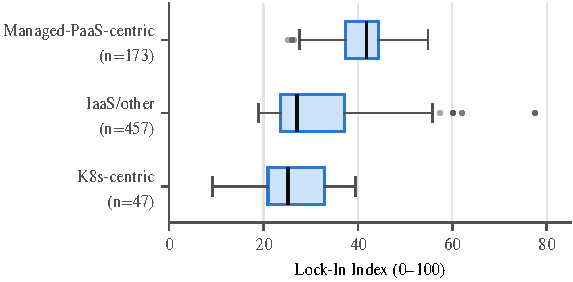
\includegraphics[width=\columnwidth]{figs/fig_groups.pdf}
\caption{LII by architectural group.}
\label{fig:groups}
\end{figure}

\begin{table}[t]
\caption{LII by architectural group. Kubernetes-centric vs.\ managed-PaaS-centric: Mann--Whitney $U=642.0$, $z=-8.85$, $p=9.0\times10^{-19}$, Cliff's $\delta=-0.84$.}
\label{tab:groups}
\centering
\footnotesize
\begin{tabular}{@{}lrrr@{}}
\toprule
Group & $n$ & Median & Mean \\
\midrule
Kubernetes-centric & 47 & 25.2 & 26.2 \\
IaaS/other & 457 & 27.1 & 31.5 \\
Managed-PaaS-centric & 173 & 41.9 & 40.8 \\
\bottomrule
\end{tabular}
\end{table}

As Fig.~\ref{fig:groups} and Table~\ref{tab:groups} show, Kubernetes-centric configurations have a median LII of 25.2 against 41.9 for managed-PaaS-centric ones, a very large effect ($\delta=-0.84$). IaaS-style configurations fall in between. The direction agrees with the conventional view that a common orchestration API reduces lock-in~\cite{burns2016,satzger2013}.

Two qualifications apply. First, Kubernetes-centric configurations are not lock-in free: their median is still about four times the score of a purely Kubernetes-native resource, because the cluster itself sits on provider networking, IAM, and node pools. Second, because the groups are defined using the same categories that the rubric scores, this result is a \emph{consistency check} that the index orders known styles sensibly; it is not independent validation against measured migration effort.

\subsection{RQ4: Robustness to Rubric Choices}

\begin{figure}[t]
\centering
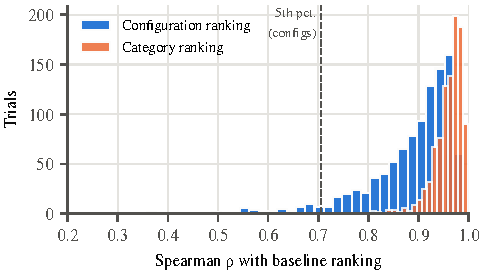
\includegraphics[width=\columnwidth]{figs/fig_sensitivity.pdf}
\caption{Spearman correlation between perturbed and baseline rankings across 1{,}000 Monte Carlo trials.}
\label{fig:sens}
\end{figure}

Fig.~\ref{fig:sens} shows that rankings are robust to moderate changes in the rubric. Across 1{,}000 trials, the configuration ranking had a median Spearman correlation of 0.91 with the baseline (5th percentile 0.71), and the category ranking a median of 0.97 (5th percentile 0.90). The Kubernetes-centric group had the lower median in 99.7\% of trials. The worst single trial ($\rho=0.25$) occurred when the sampled weights placed almost all mass on one dimension, an extreme reweighting rather than a realistic one. The overall conclusions therefore do not depend on the precise values in Table~\ref{tab:rubric}, although individual scores near the middle of the range can shift.

\section{Exit Cost: Egress and Regulation}
\label{sec:egress}

The egress dimension captures a cost that is easy to quantify. Fig.~\ref{fig:egress} applies published list prices for internet egress to a one-time exit of a given data volume. We use AWS's tiered internet rates and Azure's routing-preference rates as compiled in a July 2026 price index~\cite{egressidx}, and Google Cloud's Premium Tier rates to North America~\cite{gcpprice}; Google's tiers are in GiB, which we treat as GB for simplicity.

\begin{figure}[t]
\centering
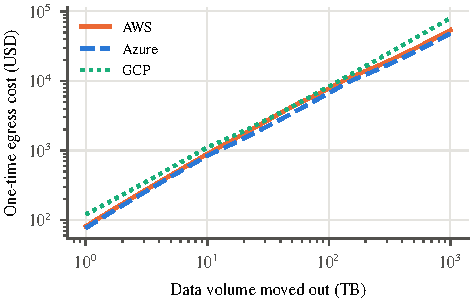
\includegraphics[width=\columnwidth]{figs/fig_egress.pdf}
\caption{One-time list-price egress cost of moving a dataset out of each provider, ignoring exit waivers. Both axes are logarithmic.}
\label{fig:egress}
\end{figure}

At 10~TB the cost is modest (\$842 on Azure, \$891 on AWS, \$1{,}110 on Google Cloud). At 100~TB it reaches \$6{,}700--8{,}300, and at 1~PB \$48{,}000--80{,}000. For most organizations, these figures are small next to the engineering effort of rewriting provider-specific code, which supports giving egress the smallest weight in the index.

The commercial landscape has also shifted. Google Cloud began offering free data transfer to customers fully leaving its platform in January 2024, subject to an approval process and a 60-day exit window~\cite{dcd2024}. AWS followed in March 2024 with credits for data transfer out when customers move away, and Microsoft announced a similar policy the same week~\cite{infoq2024}. In the EU, the Data Act (Regulation (EU) 2023/2854)~\cite{dataact} gives customers the right to switch providers, limits notice periods to two months, and allows switching charges only until January 12, 2027~\cite{dlapiper2025}. These measures lower the \emph{financial} barrier to leaving, but they do nothing about the \emph{technical} barrier---the proprietary APIs, IAM models, and data formats that dominate our index. Regulation has addressed the easy part of lock-in.

\section{Discussion}
\label{sec:discussion}

\subsection{Implications for Practitioners}
The results suggest three practical steps. \emph{First}, portability reviews should begin with identity and access management, not only with databases. Abstracting IAM is hard, but keeping policies modular and documenting the permission model in provider-neutral terms reduces rewrite effort. \emph{Second}, teams adopting managed PaaS should do so knowingly: a single proprietary NoSQL table or workflow service can raise a small configuration's score sharply, and the LII makes that trade-off visible at review time. \emph{Third}, Kubernetes lowers lock-in substantially but leaves the surrounding cloud scaffolding untouched; the cluster boundary is where most residual lock-in sits.

Because the analyzer runs on Terraform source alone, it can be added to a CI pipeline to flag pull requests that increase a configuration's LII beyond an agreed threshold, in the same way that security scanners flag misconfigurations~\cite{verdet2025}.

\subsection{The Absence of Multi-Cloud Configurations}
Not one of the 677 configurations declared resources for more than one provider. This is partly a property of the sampled repositories, most of which are provider-specific by design. Still, it is consistent with the view that ``multi-cloud'' in practice often means separate single-cloud stacks rather than applications that span providers~\cite{opara2016}. A study of private enterprise IaC would be needed to confirm this.

\subsection{Threats to Validity}
\emph{Construct validity.} The rubric scores are expert judgments by the authors, not measurements. The sensitivity analysis shows that rankings survive moderate disagreement, but the index has not yet been validated against measured migration effort. Validating it against real migrations is the most important piece of future work.

\emph{Internal validity.} The analyzer uses regular expressions rather than a full HCL evaluator. It counts every declared resource even when \texttt{count} or \texttt{for\_each} would disable it, does not expand modules fetched from registries, and assigns each resource type to one category by rule order. Manual inspection of the unclassified tail (1.3\%) suggests that misclassification is limited, but some types (for example, \texttt{azapi\_resource}, which can represent any Azure service) are inherently coarse.

\emph{External validity.} The corpus consists of examples, modules, and samples maintained by vendors and the community. These are representative of how infrastructure is \emph{taught and packaged}, but production systems may be larger and more heterogeneous. The provider comparison in RQ1 is sensitive to which repositories were sampled. Applying the analyzer to a large dataset such as TerraDS~\cite{buehler2025} would address this.

\section{Conclusion and Future Work}
This paper introduced the Lock-In Index, a transparent, rubric-based score for how tightly an IaC configuration binds an application to its cloud provider, and applied it to 677 public Terraform configurations. Lock-in turned out to be distributed throughout configurations rather than concentrated in headline services: identity, networking, and governance resources account for more than half of it, and IAM alone is the largest contributor. Kubernetes-centric designs score far lower than designs built on managed PaaS, and these conclusions hold under substantial perturbation of the rubric. Meanwhile, provider exit waivers and the EU Data Act have reduced the financial cost of leaving without touching the technical cost that the index measures.

Future work will (i) validate the index against measured migration effort by porting reference applications such as a microservice benchmark between providers, (ii) replace expert scores with values learned from documented migrations, (iii) automate cross-provider service-equivalence mapping, and (iv) scale the study to large IaC datasets and to CloudFormation and Bicep.

\section*{Data Availability}
The analyzer, rubric, and per-configuration results are provided as supplementary material. All repositories were cloned at their default branch on October 29, 2026.

\section*{Acknowledgment}
The authors used an AI assistant (Claude, Anthropic) to help draft and edit portions of the manuscript text and analysis scripts. All analysis outputs were generated by the released code, and the authors take responsibility for the content.

\bibliographystyle{IEEEtran}
\bibliography{refs}

\end{document}
